\documentclass[twocolumn,a4paper]{article}
\usepackage{graphicx}
\begin{document}
\title{Exponential-function}
\author{Wikipedia}
\maketitle


\section{Introduction}

The exponential function is widely used in mathematics and is 
represented by the letter e, which is called Euler's number, which has an 
approximate value of 2.718. The function is simply denoted 
by $e^x$ or $exp(x)$ as it lifts $e$ to the power of x. 
However, this is not the only property that the exponential function has.
When dealing with complex numbers it is used as the phase factor of a complex number.
Thus, the complex number has a modulus, i.e. the absolute value of the complex number
and it also has the beforementioned phase factor. The phase factor is what determines how much of the complex number is real and how much is imaginary.
It makes use of Euler's formula: 
\begin{equation}\label{eq:Euler}
e^{ix} = \cos(x) + i \sin(x)
\end{equation}
This is a very powerful equation and is used in physics a lot.
The definition we will use of the function here is its Taylor series:
\begin{equation}
\sum_{n=0}^{\infty} \frac{f^{(n)} (x)}{n!} = 1 + x + \frac{x^2}{2} + \frac{x^3}{6} + ...
\end{equation}

\section{Implementation}
In this paper the infinite sum will be approximated by the following function:
\begin{equation}\label{eq:approximation}
f(x) = 1+x*(1+\frac{x}{2}*(1+\frac{x}{3}*(1+\frac{x}{4}*(1+\frac{x}{5}*(1+\frac{x}{6}*(1+\frac{x}{7}*(1+\frac{x}{8}*(1+\frac{x}{9}*(1+\frac{x}{10})))))))))
\end{equation}
where the function takes the first 11 terms of the infinite sum.
In setting up the function to run in C Sharp, there needs to be two if-statements.
One is that the function should work for negative arguments. This is implemented
by saying that for x<0 then the function should return 1/f(-x), such that the
function in the denominator will have a positive argument. By the properties of
the exponential function, 1/exp(-x) corresponds to exp(x).
The other statement is, that if x>1.0/8, i.e. the shift between two x-values,
then the function should return Pow(f(x/2),2). This process lifts f(x/2) to the 
power of 2. The properties of the exponential function say that this should give
exp(x) as $exp(x/2)^2=e^x$. So this is implemented to make sure that the
approximate function works as intended, as it would diverge from the correct 
exponential function if this implementation doesn't work.

\section{Testing}
To test if the approximation works, the approximate function will be plotted
against the correct exponential function.
\begin{figure}[b]
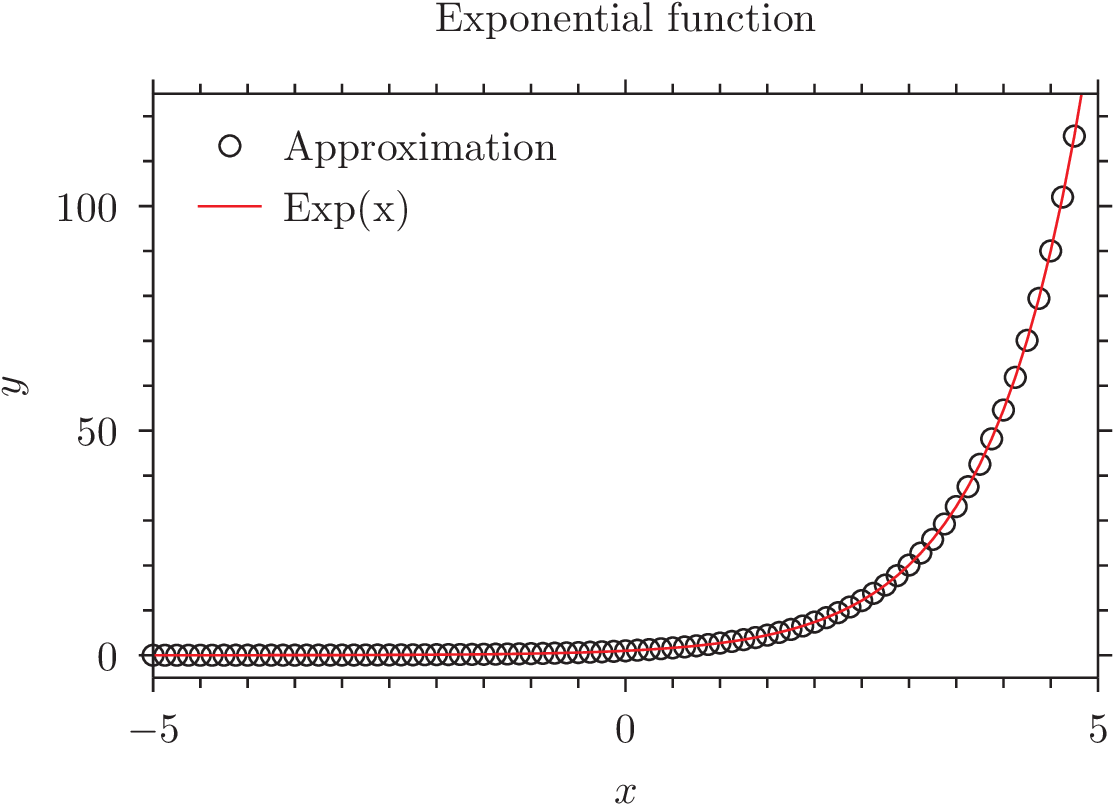
\includegraphics{exp.pyxplot.png}
\caption{Plot of the exponential function and the approximate function from this paper. The x-axis goes from -5 to 5
and the y-axis goes from -5 to 125. The red line is the exponential function and the black dots are the approximate
function. Both graphs have been created with a shift of 1.0/8 between their x-values.}
\label{fig: plot}
\end{figure}
This is plotted on figure \ref{fig: plot}. Here it can be seen that the approximate function has the same values as
correct exponential function.

\end{document}
